\chapter{Rezultate și discuții} \label{chapter:cap5} 

Acest capitol prezintă rezultatele experimentale obținute de modelul final, descris în Capitolul~\ref{chapter:cap4}, și discută semnificația acestora. Sunt prezentate, în primul rând, performanța globală a modelului pe setul de testare independent și exemple individuale de clasificare, ilustrând comportamentul acestuia pe specimene cu grade variate de încredere. Este analizată, în continuare, evoluția acurateții de-a lungul celor patru configurații experimentate, evidențiind contribuția fiecărei intervenții tehnice asupra performanței finale. Capitolul se închide cu o comparație între rezultatele obținute și abordările existente din literatură, discutate în Capitolul~\ref{chapter:cap3}.


\section{Rezultate experimentale}

Modelul final, obținut prin adaptarea arhitecturii AlexNet cu transfer learning din ImageNet și antrenat pe un set de 222 de imagini, a fost evaluat pe un set de testare independent format din 49 de imagini (28 de specimene de \textit{Austropotamobius bihariensis} și 21 de specimene de \textit{Austropotamobius torrentium}). Acuratețea obținută pe setul de testare este de \textbf{95,92\%}, corespunzând unui număr de 47 de predicții corecte din 49.

Rezultatul a fost obținut în configurația 3, care introduce extragerea automată a regiunilor de interes pe baza adnotărilor LabelMe, cu un batch size de 32 de imagini, înghețarea blocului convoluțional, normalizare ImageNet și augmentări la runtime. Selecția modelului salvat s-a realizat pe baza celei mai bune acurateți pe setul de validare, obținută în cursul celor 60 de epoci de antrenare.

Pentru a ilustra comportamentul modelului pe imagini individuale, Figura~\ref{fig:pred1}--Figura~\ref{fig:pred5} prezintă exemple reprezentative de clasificare, selectate din setul de testare utilizat la evaluarea oficială a modelului, incluzând atât predicții corecte cu grade variate de încredere, cât și cazul de clasificare incorectă identificat în Tabelul~\ref{tab:confuzie}.

\begin{figure}[H]
    \centering
    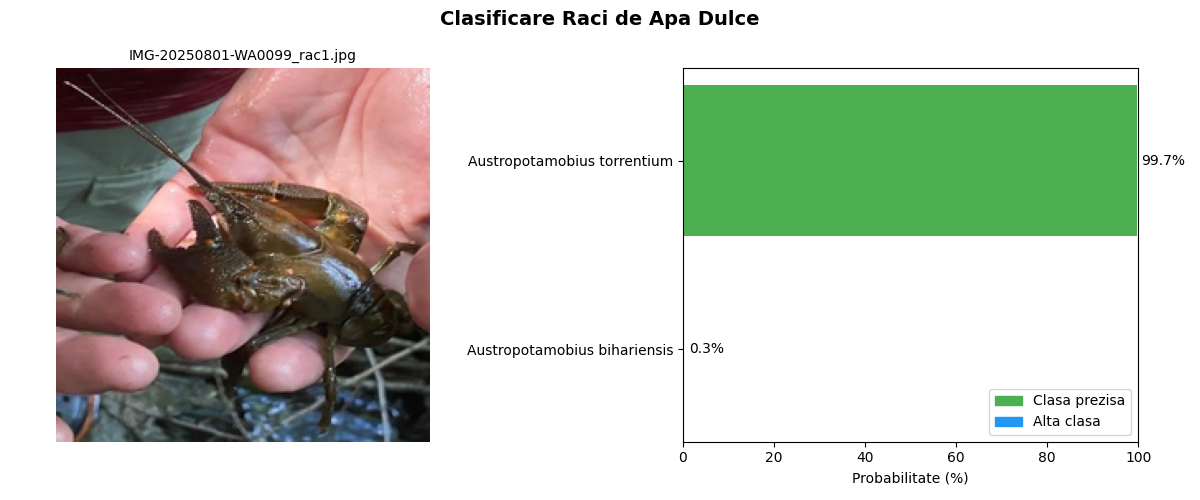
\includegraphics[width=\textwidth]{figs/Pred1_FoarteMare_Torrentium.png}
    \caption{Clasificare corectă cu încredere foarte ridicată:
    specimen de \textit{Austropotamobius torrentium} identificat
    corect cu probabilitatea de 99,7\%.}
    \label{fig:pred1}
\end{figure}

\begin{figure}[H]
    \centering
    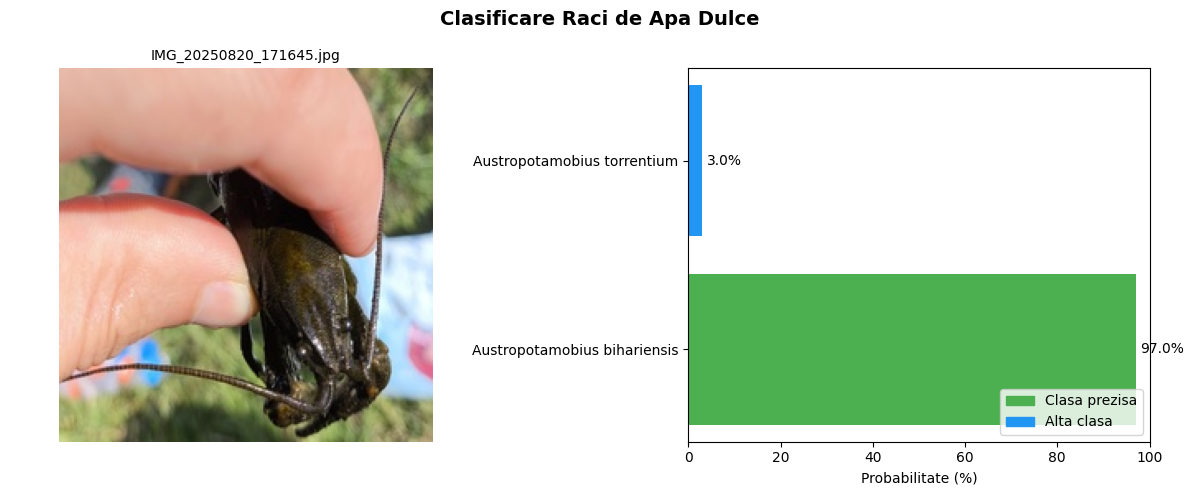
\includegraphics[width=\textwidth]{figs/Pred2_Mare_Bihariensis.png}
    \caption{Clasificare corectă cu încredere ridicată: specimen
    de \textit{Austropotamobius bihariensis} identificat corect
    cu probabilitatea de 97,0\%.}
    \label{fig:pred2}
\end{figure}

\begin{figure}[H]
    \centering
    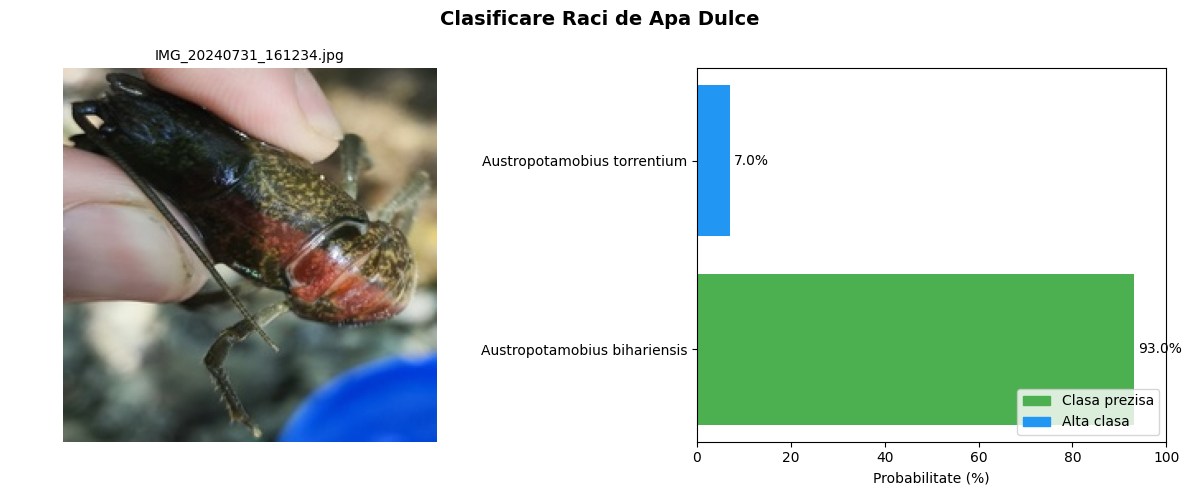
\includegraphics[width=\textwidth]{figs/Pred3_Moderata_Bihariensis.png}
    \caption{Clasificare corectă cu încredere moderată: specimen
    de \textit{Austropotamobius bihariensis} identificat corect
    cu probabilitatea de 93,0\%.}
    \label{fig:pred3}
\end{figure}

\begin{figure}[H]
    \centering
    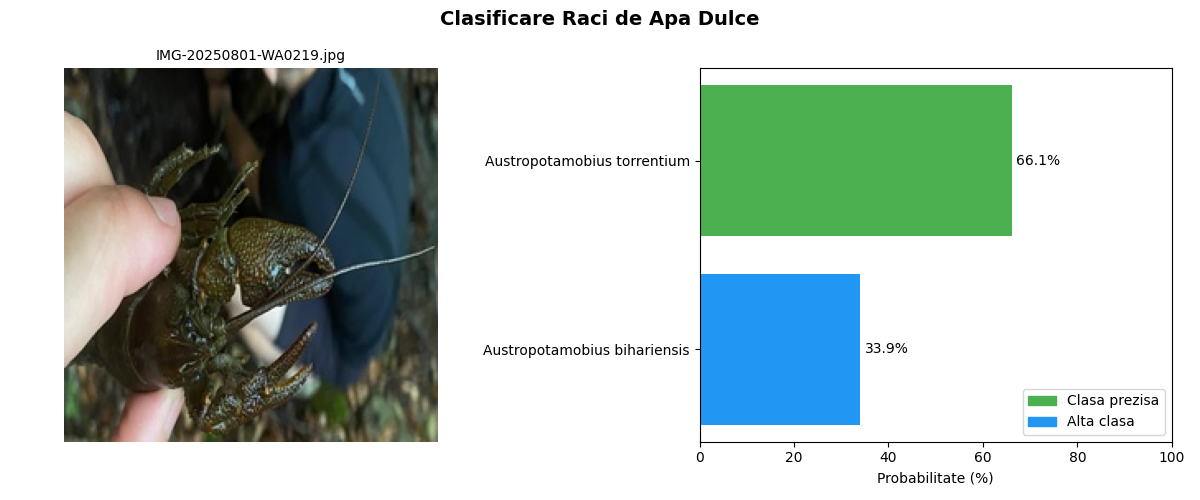
\includegraphics[width=\textwidth]{figs/Pred4_Mica_Torrentium.png}
    \caption{Clasificare corectă cu încredere scăzută: specimen
    de \textit{Austropotamobius torrentium} identificat corect
    cu probabilitatea de 66,1\%.}
    \label{fig:pred4}
\end{figure}

\begin{figure}[H]
    \centering
    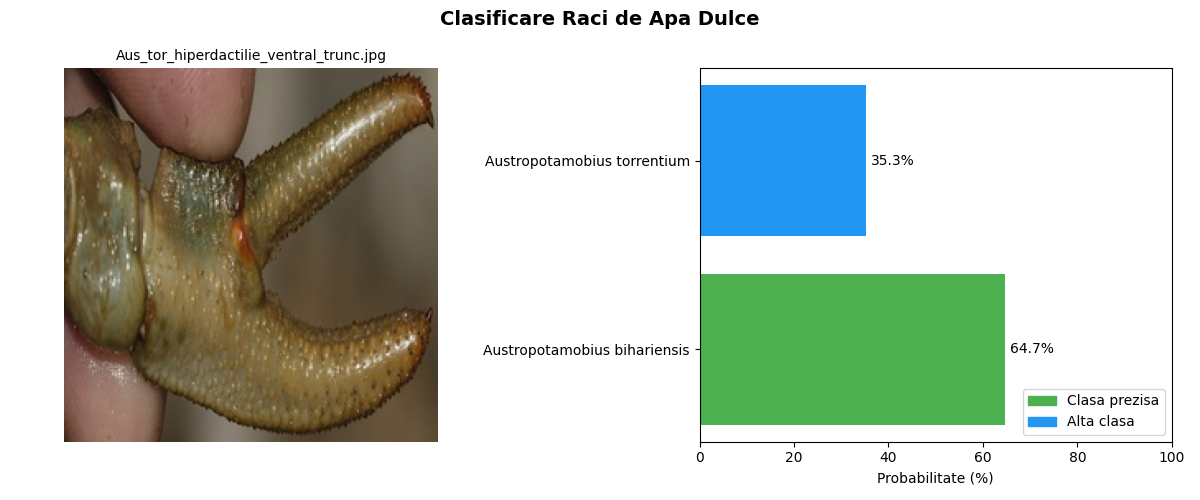
\includegraphics[width=\textwidth]{figs/Pred5_Gresit_Torrentium_ca_Bihariensis.png}
    \caption{Clasificare incorectă: specimen de \textit{Austropotamobius
    torrentium} clasificat eronat ca \textit{Austropotamobius bihariensis}
    cu probabilitatea de 64,7\%.}
    \label{fig:pred5}
\end{figure}

\section{Analiza rezultatelor}

Acuratețea de 95,92\% obținută pe setul de testare demonstrează că arhitectura AlexNet cu transfer learning este capabilă să discrimineze eficient între cele două specii de \textit{Austropotamobius} chiar și în condiții de eșantionare limitată. Evoluția performanței de-a lungul celor patru configurații experimentate relevă contribuția distinctă a fiecărei intervenții tehnice.

Primul salt major de performanță, de la 62,50\% la 87,50\%, a fost produs de introducerea înghețării blocului convoluțional, a normalizării ImageNet și a augmentărilor la runtime. Această îmbunătățire confirmă că reprezentările vizuale generale învățate de AlexNet pe ImageNet sunt suficient de expresive pentru a descrie morfologia racilor de apă dulce, fără a necesita reantrenarea convoluțiilor de la zero.

Al doilea salt major, de la 87,50\% la 95,92\%, a fost determinat de introducerea extragerii regiunilor de interes pe baza adnotărilor manuale realizate în LabelMe, urmate de decuparea automată a acestora, conform fluxului descris în Secțiunea~\ref{chapter:cap4}. Procesul nu a implicat un model de detecție automată (precum YOLO) pentru localizarea specimenelor: bounding box-urile au fost trasate manual pentru fiecare imagine, automatizarea limitându-se la etapele de decupare, redimensionare și organizare a imaginilor rezultate.

Scăderea acurateței de la 95,92\% la 93,88\% la creșterea batch size-ului de la 32 la 64 sugerează că, în contextul unui set de antrenare de dimensiuni reduse (222 de imagini), un batch size mai mic produce estimări ale gradientului mai zgomotoase dar mai reprezentative, favorizând generalizarea modelului.

\section{Comparație cu metode existente}

Lucrările prezentate în capitolul~\ref{chapter:cap3} abordează problema identificării racilor de apă dulce prin tehnici de detecție și segmentare de obiecte (YOLOv11n, YOLOv8n), pe seturi de date considerabil mai mari și pe specii diferite față de cele vizate aici. Prin natura lor, aceste metode rezolvă o problemă distinctă față de clasificarea binară propusă aici: ele localizează și delimitează specimenele în imagini de teren neprelucrate, în timp ce modelul dezvoltat în această lucrare clasifică imagini deja centrate pe specimen.

Diferența fundamentală de task (detecție și segmentare față de clasificare binară), de specii vizate și de dimensiunea seturilor de date utilizate face imposibilă o comparație numerică directă a performanțelor. Cu toate acestea, acuratețea de 95,92\% obținută pe un set de testare independent, în condițiile unui set de antrenare de doar 222 de imagini, demonstrează că abordarea prin transfer learning reprezintă o soluție viabilă pentru identificarea automată a speciilor din genul \textit{Austropotamobius} în condiții de eșantionare limitată, situație frecventă în studiile de biodiversitate pe specii protejate.



% \section{Rezultate experimentale}
% \section{Analiza rezultatelor}
% \section{Comparație cu metode existente}